\section{Techniques for CL-WSD}

%% XXX: this sentence needs some help
We will develop and extend at least two broad approaches for CL-WSD: the use
of multilingual evidence where available and sequence labeling.

Both of these techniques have been prototyped and presented at workshops, but
they will be refined significantly and integrated into a more general tool for
use in practice with MT systems.

\subsection{Using multilingual evidence}
For many languages, we have multiple bitext corpora, where each corpus covers a
different language pair. There are, for example, many bitext corpora available
for English and other languages, or for Spanish and other languages.
We would like to be able to make use of evidence from all of these corpora when
translating into any particular target language, if possible.
Each corpus may contain useful examples of a given source-language word,
and senses of that word may be lexicalized in varying, non-overlapping ways in
the different target languages.
We would want a CL-WSD system to be able to pick up on the relationships
between senses of a given word -- two target languages may happen to surface
the same sense distinctions, perhaps due to being related languages, or simply
by coincidence. Alternatively, a combination of translations into several
languages may provide evidence for a certain lexical choice in the target
language.

XXX some good examples would be good XXX

\begin{figure}
  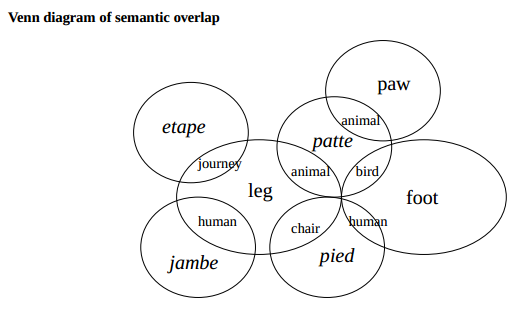
\includegraphics[width=12cm]{hutchins-leg-etc.png}
  \caption{Overlap of words related to ``leg"; relationships between English
  and French words. Translation is pretty complicated.}
  \label{fig:leg}
\end{figure}

(Figure 21.2 from Jurafsky and Martin first edition, apparently due to Hutchins
et al (XXX fix citation))
An illustrative example of the many-to-many relationship between words that are
considered translations
\cite[chap 21]{slp1}

We could also imagine using a sense-annotated corpus to train a ``monolingual"
WSD system, and use this as a 
... basically ensemble methods for WSD.

This approach is informed by the work of Lefever and Hoste
\cite{lefever-hoste-decock:2011:ACL-HLT2011}, although their technique requires
an entire machine translation system to perform CL-WSD, which is somewhat
unwieldy when we want to use CL-WSD as a subcomponent of a machine translation
system.

Earlier this year, we developed a prototype CL-WSD system that makes use of
multilingual evidence \cite{rudnick-liu-gasser:2013:SemEval-2013} and produced
some of the best results in a SemEval shared task on CL-WSD \cite{task10}.
The task was to translate polysemous nouns from English into other European
languages. In our SemEval paper, we presented three variations on the approach:
a straightforward classification approach (without multilingual evidence), a
classifier stacking approach, and a graphical model system based on loopy
belief propagation over Markov networks.

The simplest system presented in that work, based on a maximum entropy
classifier, simply extracted features from a window around the English noun to
be translated and used these to make a prediction. The same system could also
return a probability distribution over target-language words or phrases. This
simple system was used as a subcomponent in the two more sophisticated systems.

The classifier stacking approach used 
for each available bitext corpus, for each source-language word that we want to
model, we train a classifier to predict translations from the source language
into the other language of the bitext.
Then we can include the output of that classifier as a feature when training
our classifier for the desired target language.


In the graphical model approach, we treat the problem of 
... this also has the property of explicitly handling the uncertainty of each
of the component classifiers.

\subsection{Lexical selection as a sequence labeling problem}
We will also investigate the use of sequence-labeling models for lexical
selection.  The intuition behind the sequence-labeling approach is that machine
translation implies an ``all-words" WSD task, in that we need to choose a
translation for every word or phrase in the source sentence, and that the
sequence of translations chosen should make sense when taken together.

One promising formalism for this line of work is the Maximum Entropy Markov
Model \cite{icml00/mccallum}, which can be combined in a straightforward way
with the simpler Hidden Markov Model (HMM).
This combination allows for efficient inference and the ability to trade more
computational resources for richer modeling. More sophisticated sequence
models, such as Conditional Random Fields, may be useful in this task as well.

We also developed a prototype CL-WSD system based on sequence labeling and
applied it to both English-Spanish and Spanish-Guarani translation tasks; this
work was presented at the HyTra workshop in August
\cite{rudnick-gasser:2013:HyTra-2013}.

For the sequence labeling approach in which only some words have their
translations modeled explicitly with a classifier, we have yet to explore what
the best approaches are for choosing \emph{which} words should get classifiers.

We will also look into the best ways to integrate the multilingual approach
with this one.

\subsection{Applying similar techniques for morphology prediction}

Sequence labeling has also been applied to the problem of generating
morphological features in target language text, so that target language output
words are appropriately inflected...
\cite{toutanova-suzuki-ruopp:2008:ACLMain}

This will be one of the approaches we investigate in the development of
Tereré...

